
We examine numerically the boundaries in finite dimensions, illustrating the boundary \eqref{eq:strong-classification-boundary} under several error tail assumptions, as well as error dependence structures.

\subsection{Exact support recovery and tail assumptions}

To demonstrate the phase-transition phenomenon under different error tail densities, we simulate from the additive error model \eqref{eq:model} with
\begin{itemize}
    \item Gaussian errors, where the density is given by
    $$f(x) = \frac{1}{\sqrt{2\pi}}\exp{\left\{-x^2/2\right\}}.$$
    \item Laplace errors, where the density is given by $$f(x) = \frac{1}{2}\exp{\left\{-\left|x\right|\right\}}.$$
    \item Generalized Gaussian errors with $\nu=1/2$, where the density is given by 
    $$f(x) = \frac{1}{2}\exp{\left\{-2\left|x\right|^{1/2}\right\}}.$$
\end{itemize}
The sparsity and signal size of the sparse mean vector are parametrized as in equations \eqref{eq:sparsity-parametrized} and \eqref{eq:signal-size-parametrized}, respectively.
The support set $S$ is estimated with 
$\widetilde{S} = \left\{j:x(j)>\sqrt{2\log{p}}\right\}$ 
under the Gaussian errors, 
$\widetilde{S} = \left\{j:x(j)>\log{p} + (\log{\log{p}})/2\right\}$ 
under the Laplace errors, and with
$\widetilde{S} = \{j:x(j)> \frac{1}{4}\left(W\left(-c/(ep\log{p})\right) + 1\right)^2\}$
under the generalized Gaussian ($\nu = 1/2$) errors. Here $W$ is the Lambert W function, i.e., $W=f^{-1}$ where $f(x)=x\exp{(x)}$.
The choices of thresholds correspond to Bonferroni's procedures with FWER decreasing at a rate of $1/\sqrt{\log{p}}$, therefore satisfying the assumptions in Theorem \ref{thm:sufficient}.
Experiments were repeated 1000 times under each sparsity-and-signal-size combination.

The results of the numerical experiments are shown in Figure \ref{fig:phase-simulated}.
The numerical results illustrate that the predicted boundaries are not only accurate in high-dimensions ($p=10000$, right panels of Figure \ref{fig:phase-simulated}), but also practically meaningful even at moderate dimensions ($p=100$, left panels of Figure \ref{fig:phase-simulated}).

\begin{figure}
      \centering
      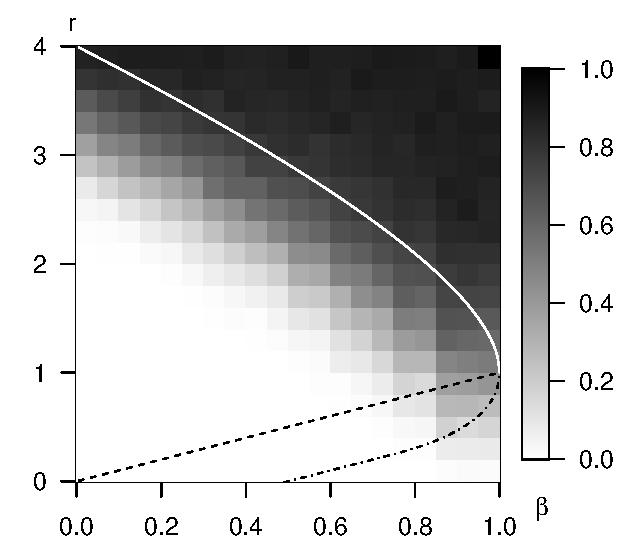
\includegraphics[width=0.4\textwidth]{./figures/simulated_phase_diagram_p100.eps}
      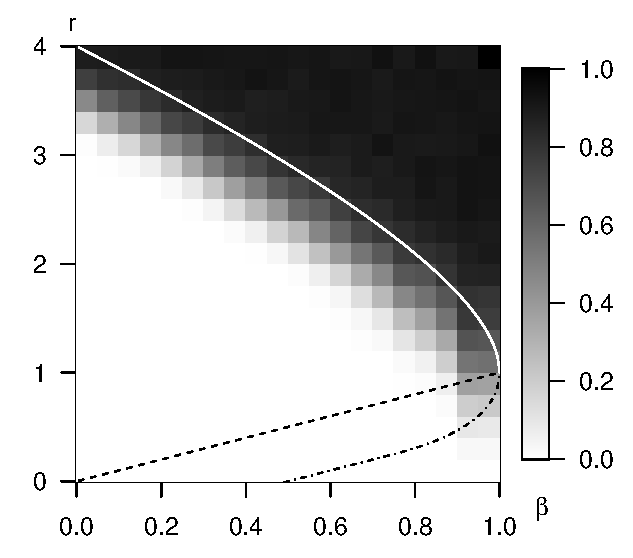
\includegraphics[width=0.4\textwidth]{./figures/simulated_phase_diagram_p10000.eps}
      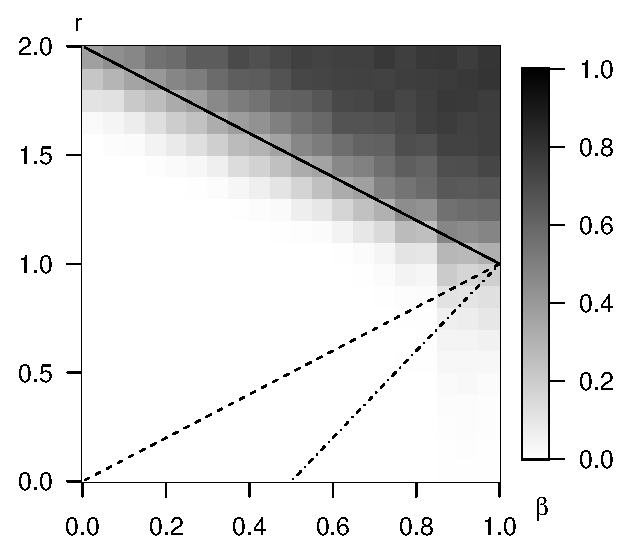
\includegraphics[width=0.4\textwidth]{./figures/simulated_phase_diagram_Laplace_p100_4.eps}
      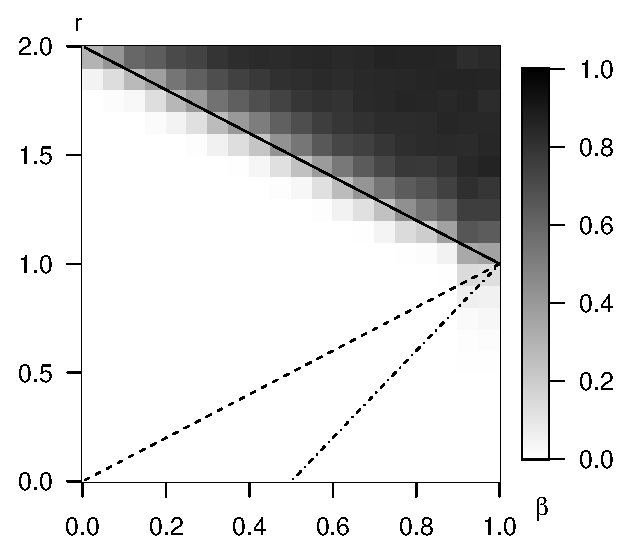
\includegraphics[width=0.4\textwidth]{./figures/simulated_phase_diagram_Laplace_p10000_4.eps}
      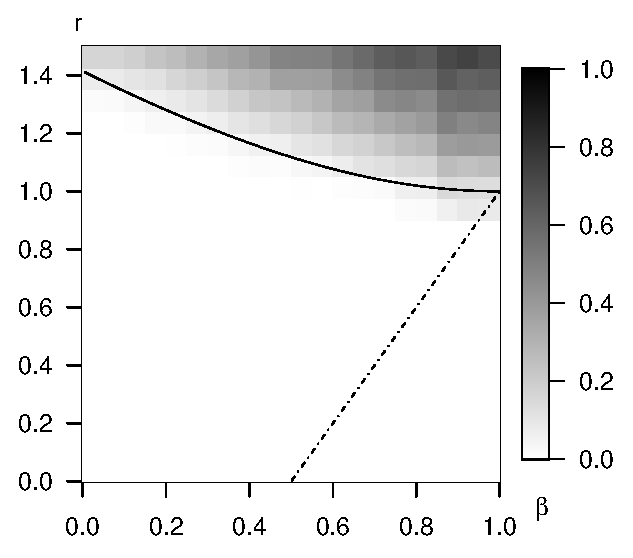
\includegraphics[width=0.4\textwidth]{./figures/simulated_phase_diagram_NLC_p100.eps}
      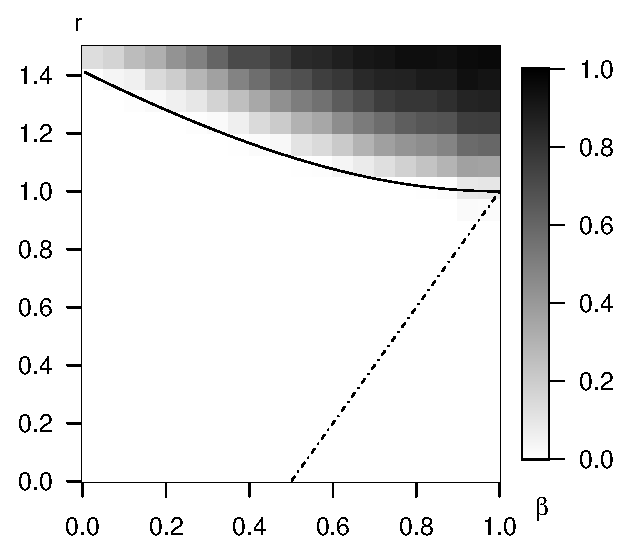
\includegraphics[width=0.4\textwidth]{./figures/simulated_phase_diagram_NLC_p10000.eps}
      \caption{The empirical probability of exact support recovery from numerical experiments, as a function of sparsity level $\beta$ and signal sizes $r$, from Gaussian error models (upper panels), Laplace error models (middle panels), and generalized Gaussian with $\nu=1/2$ (lower panels); darker color indicates higher probability of exact support recovery. 
      The experiments were repeated 1000 times for each sparsity-signal size combination, and for dimensions $p=100$ (left panels) and $p=10000$ (right panels). Numerical results agree with the boundaries described in Theorem \ref{thm:sufficient}; convergence is noticeably slower for under generalized Gaussian ($\nu=1/2$) errors.
      For reference, the dashed and dash-dotted lines represent the weak classification and detection boundaries (see Sec \ref{sec:sufficient}, and \citep{haupt2011distilled, arias2017distribution, ingster1998minimax, donoho2004higher}).}
      \label{fig:phase-simulated}
\end{figure}

\subsection{Exact support recovery and dependence}

We also illustrate the effect of dependence on the phase-transition behavior in finite dimensions.
We shall compare the performance of the sparsity- and signal-size-agnostic Bonferroni's procedure with the oracle procedure which picks the top-s observations.

The first set of experiment simulates dependent errors from an auto-regressive (AR) model.
\begin{itemize}
    \item AR(1) Gaussian errors with parameter $\rho = -0.5$, $\rho = 0.5$, and $\rho = 0.9$,
    where the autocovariance functions decay exponentially
    $$\rho_{k} = \rho^{k}.$$
\end{itemize}
The results of the experiment are shown in Figure \ref{fig:phase-simulated-dependent}.

The second set of experiments explores heavily dependent, and non-UDD errors.
In particular we simulate
\begin{itemize}
    \item Fractional Gaussian noise (fGn) with Hurst parameter $H = 0.75$ and $H = 0.9$. 
    The autocovariance functions are 
    % $$\rho_{k} \sim 2H(2H-1)k^{2H-2},$$
    $$\rho_{k} \sim 0.75k^{-0.6},$$
    and, respectively,
    $$\rho_{k} \sim 1.44k^{-0.2},$$
    as $k\to\infty$.
    Both fGn models represent the regime of long-range dependence, where covariances decay very slowly to zero, so that $\sum|\rho_k| = \infty$.
    \item The non-UDD Gaussian errors described in Example \ref{exmp:counter-example}.
\end{itemize}
We will apply both the the sparsity- and signal-size agnostic Bonferroni's procedure, i.e., $\widetilde{S} = \{j:x(j)>\sqrt{2\log{p}}\}$, as well as the oracle procedure $\widehat{S}^* = \{j:x(j)\ge x_{[s]}\}$, $s=|S|$, to all settings.
Results of the numerical experiments for the AR models are shown in Figure \ref{fig:phase-simulated-dependent}; the fGn and non-UDD models are shown in Figure \ref{fig:phase-simulated-very-dependent}.

Notice that the oracle procedure sets its thresholds more aggressively (at roughly $\sqrt{2\log s}$) than the Bonferroni procedure (at $\sqrt{2\log p}$).
Although this difference vanishes as $p\to\infty$, in finite dimensions ($p=10\,000$) the advantage can be felt. 
Indeed, in all our experiments the oracle procedures is able to recover support of signals with higher probability than the Bonferroni procedures; compare left and right columns of Figures \ref{fig:phase-simulated-dependent} and \ref{fig:phase-simulated-very-dependent}.
Notice also that there is an increase in probability of recovery near $\beta=0$ for oracle procedures.
This is an artifact due to the fact that $s = \lfloor p^{1-\beta}\rfloor < p/2$, and there are more signals than nulls. The oracle procedures is able to adjust to this reversal by lowering its threshold accordingly.

For UDD errors, Theorem \ref{thm:necessary} predicts that exact recovery of the support is impossible when signal sizes are below the boundary \eqref{eq:strong-classification-boundary}, even with oracle procedures. 
Both the AR and the fGn models generate UDD Gaussian errors, and should demonstrate the same phase-transition boundary.
However, the rate of this convergence (i.e., $\P[\widehat{S}^*=S]\to0\;\text{or}\;1$) can be very slow when the errors are heavily dependent,
even though all AR and fGn models demonstrate qualitatively the same behavior in line with the predicted boundary \eqref{eq:strong-classification-boundary}. 
In finite dimensions ($p=10\,000$), as dependence in the errors increases (AR(1) to fGN(H=0.9)), the oracle procedure becomes more powerful at recovering signal support with high probability for weaker signals. 
See right columns of Figures \ref{fig:phase-simulated-dependent} and \ref{fig:phase-simulated-very-dependent}.

On the other hand, as demonstrated in Example \ref{exmp:counter-example}, non-UDD errors yield qualitatively different behavior; exact recovery of support is possible for signal sizes strictly weaker than that in the UDD case. 
Lower-right panel of Figure \ref{fig:phase-simulated-very-dependent} demonstrates in this example that the signal support can be recovered as long as the signal sizes are larger than $4(1-\beta)$.

\begin{figure}
    \centering
    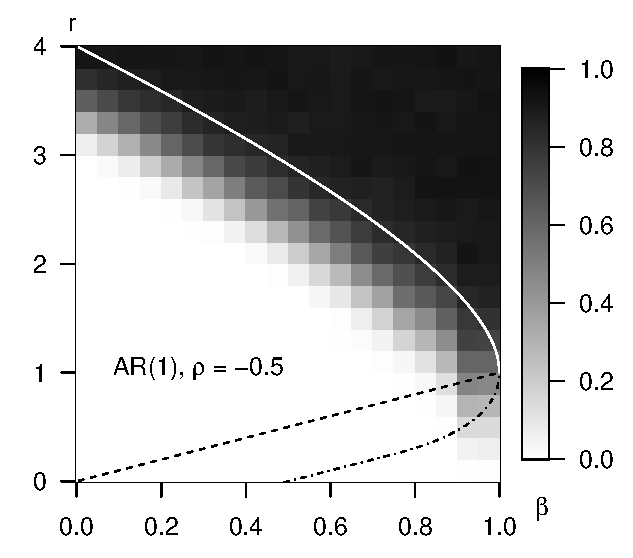
\includegraphics[width=0.4\textwidth]{./figures/simulated_phase_diagram_AR-05_p10000.eps}
    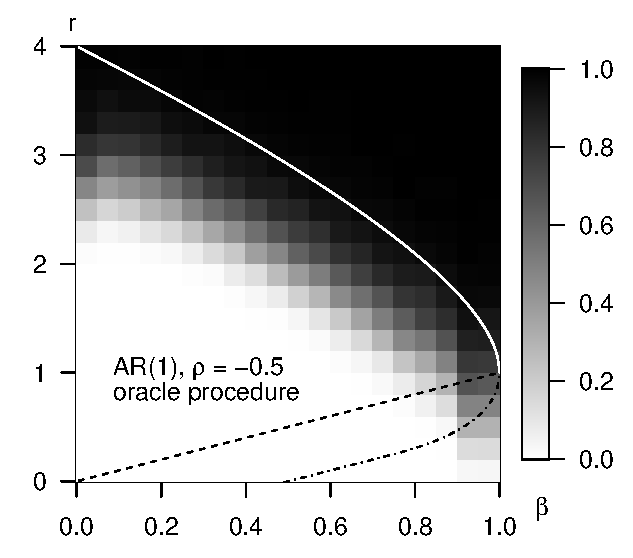
\includegraphics[width=0.4\textwidth]{./figures/simulated_phase_diagram_AR-05_p10000_oracle.eps}
    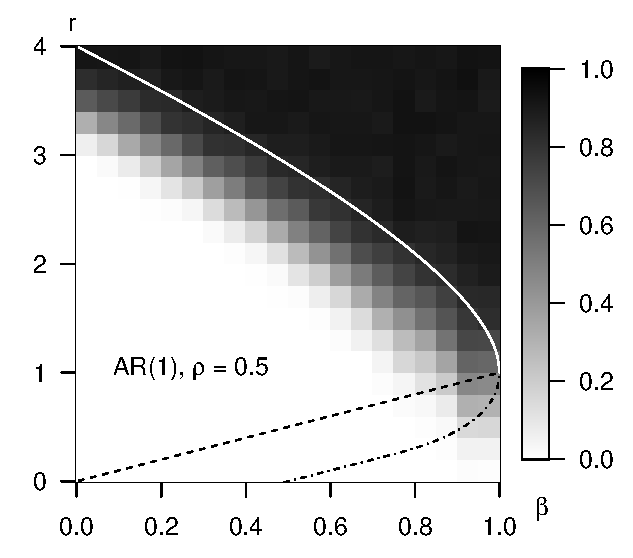
\includegraphics[width=0.4\textwidth]{./figures/simulated_phase_diagram_AR05_p10000.eps}
    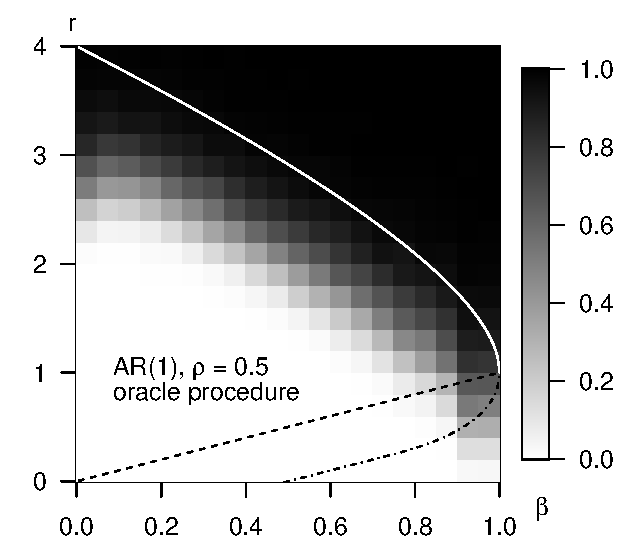
\includegraphics[width=0.4\textwidth]{./figures/simulated_phase_diagram_AR05_p10000_oracle.eps}
    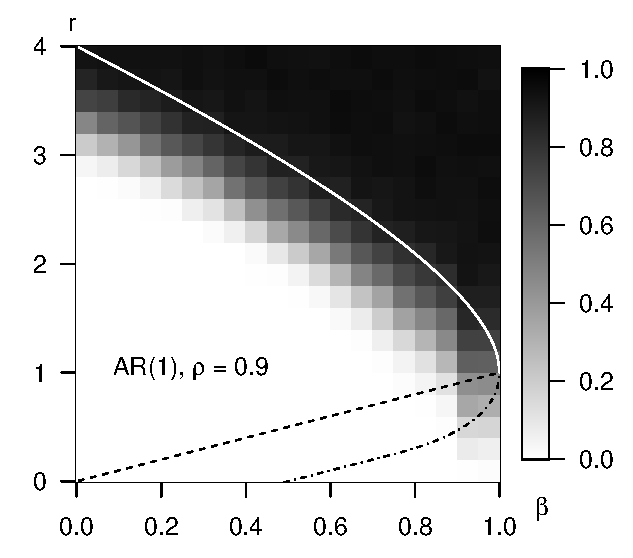
\includegraphics[width=0.4\textwidth]{./figures/simulated_phase_diagram_AR09_p10000.eps}
    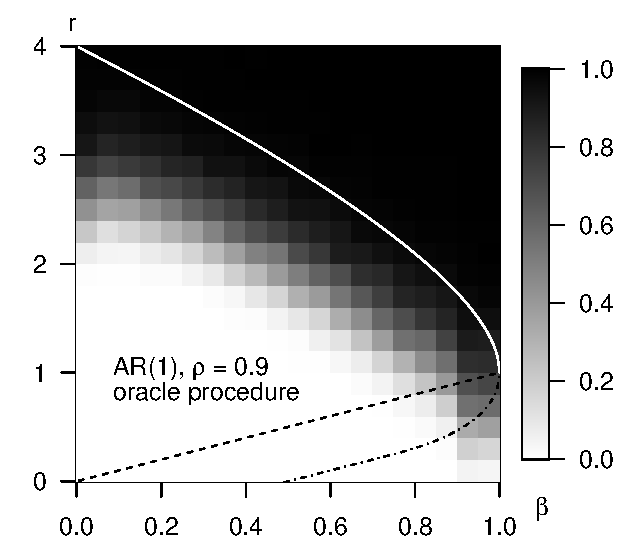
\includegraphics[width=0.4\textwidth]{./figures/simulated_phase_diagram_AR09_p10000_oracle.eps}
    \caption{The empirical probability of exact support recovery from numerical experiments, as a function of sparsity level $\beta$ and signal sizes $r$. Darker colors indicate higher probability of exact support recovery. 
    Three AR(1) models with autocorrelation functions $(-0.5)^k$ (upper), 
    $0.5^k$ (middle), and $0.9^k$ (lower) are simulated.
    The experiments were repeated 1000 times for each sparsity-signal size combination.
    In finite dimensions ($p=10000$), the Bonferroni procedures (left) suffers small loss of power compared to the oracle procedures (right).
    A phase-transition in agreement with the predicted boundary \eqref{eq:strong-classification-boundary} can be seen in the AR models.
    The boundaries (solid, dashed, and dash-dotted lines) are as in Fig \ref{fig:phase-simulated}.
    See text for additional comments.}
    \label{fig:phase-simulated-dependent}
\end{figure}

\begin{figure}
    \centering
    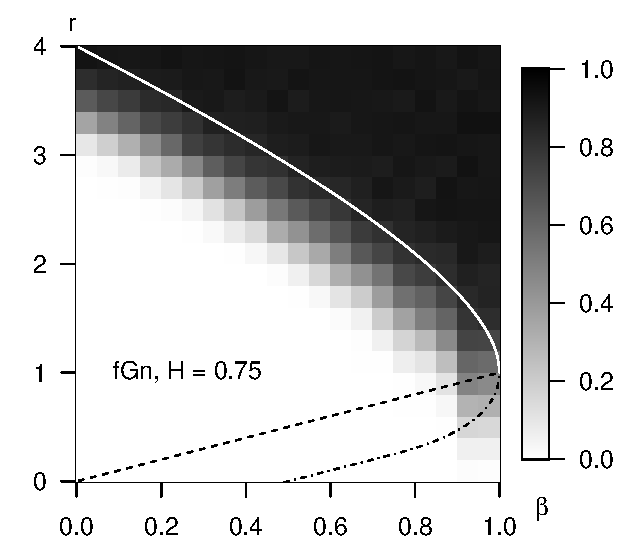
\includegraphics[width=0.4\textwidth]{./figures/simulated_phase_diagram_fGn075_p10000.eps}
    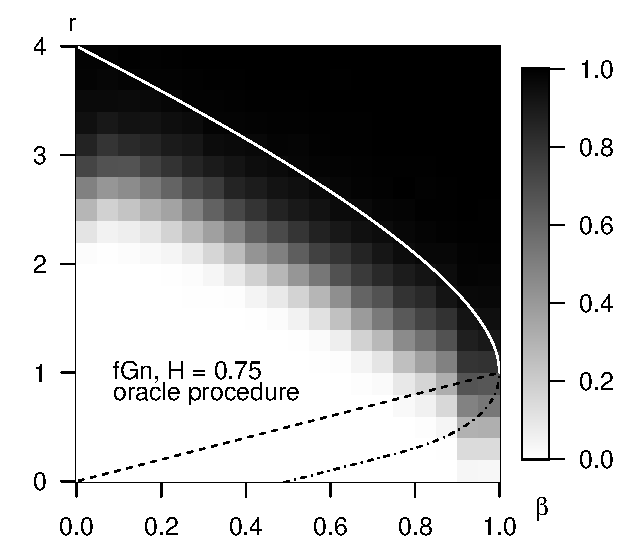
\includegraphics[width=0.4\textwidth]{./figures/simulated_phase_diagram_fGn075_p10000_oracle.eps}
    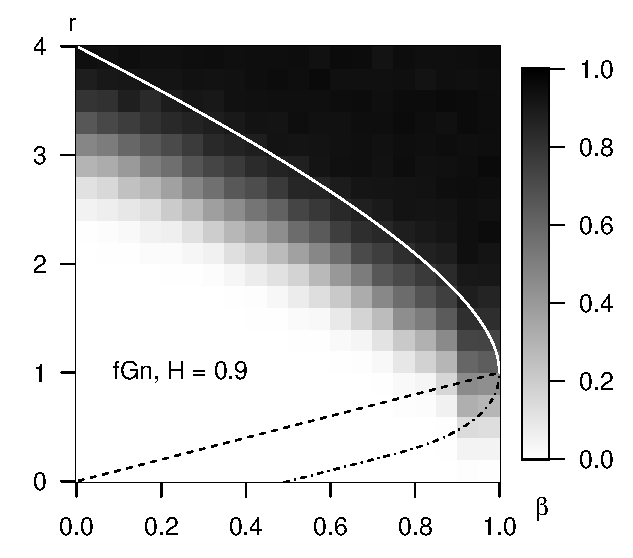
\includegraphics[width=0.4\textwidth]{./figures/simulated_phase_diagram_fGn09_p10000.eps}
    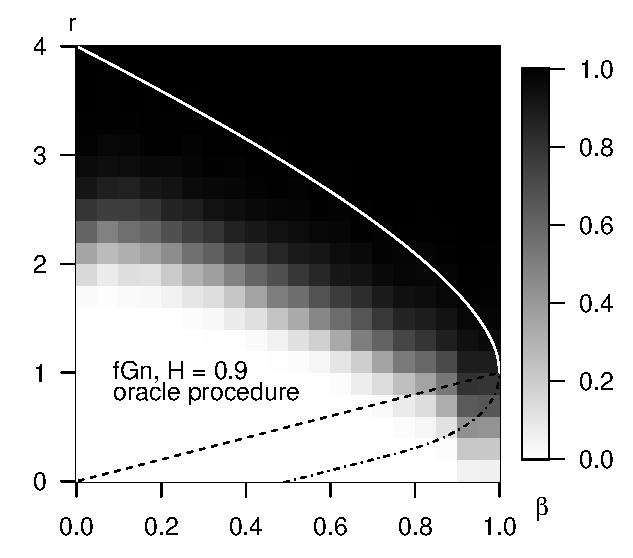
\includegraphics[width=0.4\textwidth]{./figures/simulated_phase_diagram_fGn09_p10000_oracle.eps}
    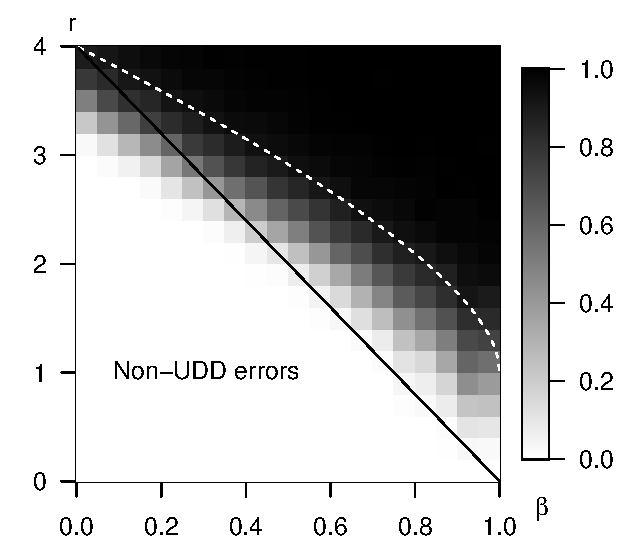
\includegraphics[width=0.4\textwidth]{./figures/simulated_phase_diagram_block_structure_p10000_agnostic7.eps}
    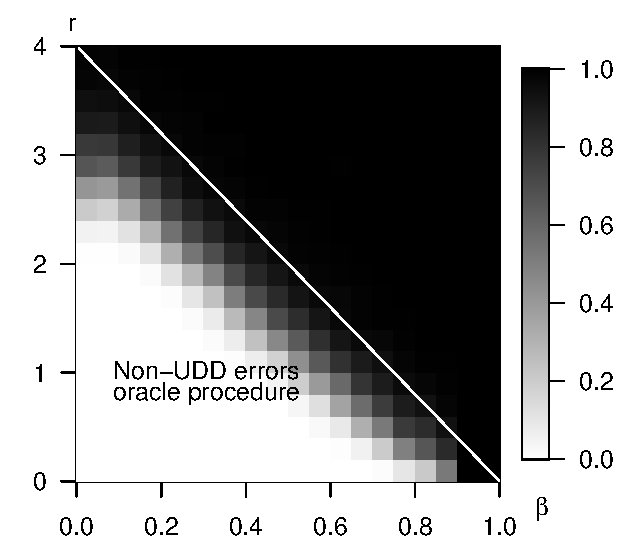
\includegraphics[width=0.4\textwidth]{./figures/simulated_phase_diagram_block_structure_p10000_oracle6.eps}
    \caption{The empirical probability of exact support recovery from numerical experiments, as a function of sparsity level $\beta$ and signal sizes $r$. Darker colors indicate higher probability of exact support recovery. 
    Two fGn models with Hurst parameter $H = 0.75$ (upper), 
    $H = 0.9$ (middle), and the non-UDD errors in Example \ref{exmp:counter-example} (lower) are simulated.
    The experiments were repeated 1000 times for each sparsity-signal size combination.
    In finite dimensions ($p=10000$), the oracle procedures (right) is able to recover support for weaker signals than the Bonferroni procedures (left) when errors are heavily dependent, although they have the same phase-transition limit.
    The non-UDD errors demonstrates qualitatively different behavior, enabling support recovery for strictly weaker signals.
    The boundaries (solid, dashed, and dash-dotted lines) are as in Fig \ref{fig:phase-simulated}.
    In the non-UDD example, dashed lines represent the limit attained by Bonferroni's procedures.
    See text for additional comments.}
    \label{fig:phase-simulated-very-dependent}
\end{figure}